
\documentclass[11pt]{amsbook}

\usepackage{../HBSuerDemir}	% ------------------------


\begin{document}

% ++++++++++++++++++++++++++++++++++++++
\hPage{b1p1/21}

$$A\subseteq B \ and \ B\subseteq A  \ \Longleftrightarrow \ A=B$$

\par \ \par This implication can be used to prove equality of sets.

Some subsets of R are in so frequent use that they bear special symbols, namely:

$$R^+=\{x: \ x>0,x\in R \}, \ R^-=\{x: \ x<0,x\in R \}, \ R^*=\{x: \ x\in R,x\neq 0 \}$$

In the same way we may talk about the subsets of $\mathbb{Q}$, $\mathbb{Z}$ and $\mathbb{N}$ (Why $\mathbb{N}^-=\emptyset$ ? However some authors use $\mathbb{N}^-$ for $\mathbb{Z}^-$. In our notation, $\mathbb{N}^-$ is the set of all negative elements of $\mathbb{N}$, which is the empty set.)

\begin{enumerate}
  \item[C.] \underline{Operations with sets}
\end{enumerate}

Given two sets A and B, by means of three operations "$\cap$", "$\cup$" and "$\setminus$" we define the three sets, namely

\begin{enumerate}
  \item $A\cap B=\{ x: x\in A \ and \ x\in B\}$  "A intersection B"
  \item $A\cup B=\{ x: x\in A \ or \ x\in B\}$  "A union B"
  \item $A\setminus B=\{ x: x\in A,\ x\not \in B\}$  "A minus B"
\end{enumerate}

Venn diagrams of these sets are indicated by shaded sets given below:

\par \ 

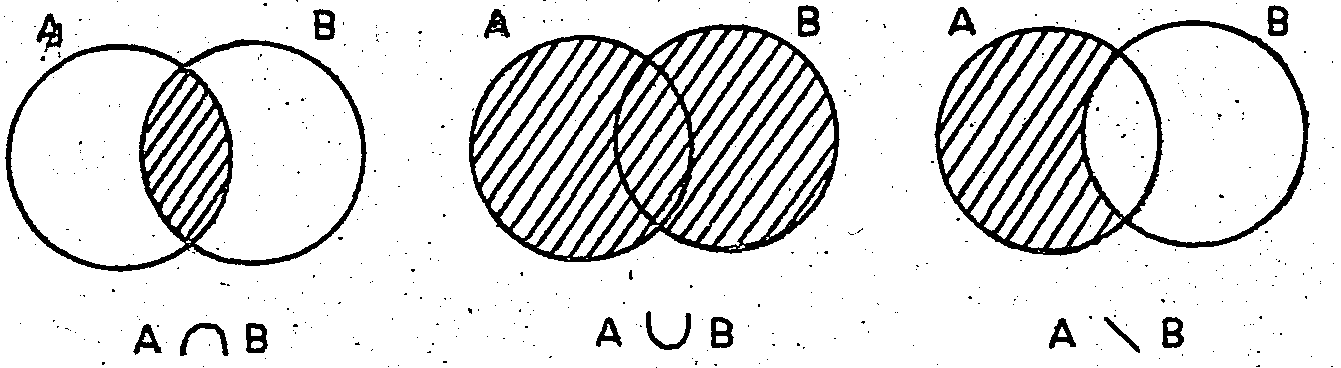
\includegraphics[scale=0.3]{images/b1p1-021-fig01}

\end{document}  

